\chapter{Transactional Clustering}

Clustering is a task whose objective is to find grouping of objects of a dataset into sets, called clusters, where each member of a cluster is more similar to all other elements in the same cluster than it is to elements in different clusters. For numerical data, proximity between objects is measured using distances, typically Euclidean or Manhattan, since records with numerical attributes only can be interpreted as points in an $n$ dimensional space. However, these measures are not appropriate to carry clustering tasks on categorical attributes, which are used to represent transactional data. The biggest issue is that the way two transactions are deemed ``near'' each other does not correspond to geometrical proximity.

This issue can be illustrated with a simple example. Assume we have 4 transactions:
\begin{align*}
    &T1 = \{1,2,3,4\} \\
    &T2 = \{1,2,4\} \\
    &T3 = \{3\} \\
    &T4 = \{4\}
\end{align*}
Usually, transactional data can be represented with a set of boolean attributes, one for each item, where a value of ``1'' indicates the presence of the corresponding item, while a ``0'' indicates its' absence. In this case, the dataset will be represented as:
\begin{align*}
    &P1 = \{1,1,1,1\} \\
    &P2 = \{1,1,0,1\} \\
    &P3 = \{0,0,1,0\} \\
    &P4 = \{0,0,0,1\} \\
\end{align*}
If Euclidean distance were used to calculate how far or close there transactions are to each other, we would find out that the distance between transactions 3 and 4 is:
\begin{equation*}
    d(P3, P4) = \sqrt{(0)^2 + (0)^2 + (1)^2 + (-1)^2} = \sqrt{2}    
\end{equation*}
However, the two transactions don't share any item, making them completely different.

This chapter will present four different algorithms that can cluster categorical data, each of which define proximity between transactions in different ways.

\section{K-Modes}

K-modes is similar to K-means, but can be used for categorical attributes. It starts by randomly choosing $k$ data points at random to elect to representative points. The algorithm then enters a loop, in which it assigns all points to the closest mode, recomputes the mode of each cluster, and repeats the past two steps until no object changes assignment between two successive iterations (or until some stopping criterion is verified).

The distance between two records is calculated as the number of mismatches between their attributes:
\begin{gather*}
    d(X,Y) = \sum_i \delta(x_i, y_i) \\
    \delta(x,y) = \begin{cases}
        0 & (x = y) \\
        1 & else
    \end{cases}
\end{gather*}
The representative object of a cluster is calculated as the mode of the objects in the same cluster.

This algorithm minimizes the function:
\begin{equation*}
    P(W,Q) = \sum_{i}^k \sum_{j}^n w_{i,j} d(x_i, Q_i) \,,
\end{equation*}
where $w_{i,j}$ is 1 if object $i$ belongs to cluster $j$, 0 otherwise, and $Q$ is the set of the modes of each cluster.

\section{ROCK (RObust Clustering using linK)}

ROCK is a hierarchical algorithm that uses \textbf{neighborhoods} and \textbf{links to clusters} to define closeness between two transactions. Neighborhoods are calculated locally, while links are calculated globally. The algorithm can be split into three main parts:
\begin{enumerate}
    \item \textbf{A random sample is drawn from the dataset}. A sample of points is uniformly extracted, using it to form clusters instead of the entire data. This ensures the algorithm can be used even on very large dataset while still producing an accurate enough clustering.

    \item \textbf{An agglomerative hierarchical clustering algorithm is performed on the sample}. ROCK follows the same steps as other hierarchical agglomerative algorithms: it starts by assigning each point to a singleton cluster, then computes the similarity measure for all pairs of clusters, and merges the two ``closest'' objects. These steps repeat until some stopping condition is met (usually, until $k$ clusters are formed).

    Two objects $A$ and $B$ are \textbf{neighbors} if their similarity is greater or equal than some hyperparameter threshold $\theta$, chosen between 0 and 1:
    \begin{equation*}
        A \in N_B \land B \in N_A \iff sim(A,B) \geq \theta \,,
    \end{equation*}
    where similarity is calculated with Jaccard's coefficient (the ratio of the number of matching items between the objects and the total number of distinct items between the two):
    \begin{equation*}
        sim(A,B) = \dfrac{|A \cap B|}{|A \cup B|}
    \end{equation*}
    A point is also considered a neighbor of itself.

    A \textbf{link} is calculated as the number of common neighbors between two objects:
    \begin{equation*}
        link(A,B) = |N_A \cap N_B|
    \end{equation*}
    Higher values of link means that there's a higher probability that the two objects belong to the same group (since they share neighbors). 
    
    \item \textbf{The entire dataset is labeled by assigning each object to a cluster}. A random sample is selected from each cluster, and each point $p$ in the original dataset is assigned to the cluster $i$ such that $p$ has the maximum number of neighbors in the corresponding sample.
\end{enumerate}
The best clusters are the ones that maximize the criterion function of the algorithm:
\begin{align*}
    &E_l = \sum_{i=1}^k n_i \sum_{p_q,p_r \in C_i} \dfrac{link(p_q, p_r)}{n_i^{1 + 2 f(\theta)}} \,, \\
    & f(\theta) = \dfrac{1-\theta}{1+\theta}
\end{align*}
where $n_i$ is the size of cluster $C_i$. This function penalizes clusters that present very few links compared to the expected number of links in the entire cluster, so that we avoid that objects with a low number of links are assigned to the same cluster. At each merging step of the algorithm, the two clusters that are merged are the ones that maximize the goodness measure:
\begin{equation*}
    g(C_i, C_j) = \dfrac{link(C_i, C_j)}{(n_i + n_j)^{1+2f(\theta)} - n_i^{1+2f(\theta)} - n_j^{1+2f(\theta)}} \,,
\end{equation*}
where the numerator is the number of cross-links between the two clusters, and the denominator is the expected number of them.

\section{CLOPE (Clustering with sLOPE)}

CLOPE is a clustering algorithm that is efficient for high dimensional data. It uses an exclusively global criterion function that tries to increase the intra-cluster overlap of transactions. This is done by increasing the height-to-width ratio of the cluster histogram. It is especially suitable for big datasets with a high number of unique items, since it uses an array representation of the data instead of binary.

For each cluster, the width is calculated as the number of distinct items, while the height is calculated as the ratio between the total number of (non unique) items and the width. In the example below, the cluster has a width of 5 and a height of 2.4.
\begin{figure}[h]
    \centering
    \begin{minipage}{0.49\textwidth}
    \centering
    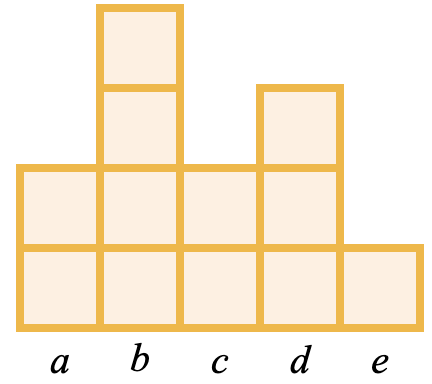
\includegraphics[width=0.5\linewidth]{img/CLOPE_cluster.png}
    \begin{equation*}
        C_i = \{abcd, bcd, ab, bde\}
    \end{equation*}
    \end{minipage}
\hfill
    \begin{minipage}{0.49\textwidth}
        \begin{gather*}
            W(C_i) = 5 \\
            S(C_i) = 12 \\
            H(C_i) = \dfrac{12}{5} = 2.4
        \end{gather*}
    \end{minipage}
\end{figure} \\
Higher ratios of height/width mean higher item overlapping.

The goodness of a clustering is calculated as the \textbf{gradient} of each cluster:
\begin{equation*}
    \textit{Profit}_r(C) = \dfrac{\sum_{i=1}^k \dfrac{S(C_i)}{W(C_i)^r} \times |C_i|}{\sum_{i=1}^k |C_i|}
\end{equation*}
The hyperparameter $r$ is called \textbf{repulsion}; for higher values of $r$, transactions within the same cluster must share a large portion of items, while for lower values transactions may share a lower amount of items, which can be useful for sparse databases.

The algorithm has two phases: first, each transaction is added to a new cluster or to an existing one such that the profit is maximized. Then, for each transaction, it is checked whether moving it to a different cluster improves profit, repeating this step until all transactions remain in the same cluster (no moves will improve the profit).

\section{TX-Means}

TX-Means is a parameter-free transactional clustering algorithm, and is useful to partition data obtained from a massive amount of different datasets. It finds a representative transaction for each cluster, which summarizes the pattern presented by the elements of that cluster. Like X-Means, it starts out with a cluster that contains all the objects in the dataset, and chooses how to recursively split it into subpartitions by using the Bayesian Information Criterion.
\begin{algorithm}
\caption{TX-Means pseudocode.}
\begin{algorithmic}[1]
    \State $r$ = \texttt{getRepr}($B$) \# get representative basket of entire set of baskets
    \State $r$ is added to queue $Q$

    \While{$Q \neq \emptyset$}
        \State $C, r$ are extracted from $Q$
        \State Common items are removed from $C$ and $r$
        \State $C1,C2,r1,r2$ = \texttt{bisectBasket}($C$)
        \If{$\textit{BIC}(C1,C2,r1,r2) > \textit{BIC}(C,r)$}
            \State Add $C1,C2,r1,r2$ to $Q$
        \Else
            \State Add $C, r$ to result 
        \EndIf
    \EndWhile

    \State Return result
\end{algorithmic}
\end{algorithm} \\
The algorithm starts by finding a representative for all objects in the dataset, then enters a loop in which each cluster currently in the queue is split. Each split is either accepted, reinserting the new subpartitions in the queue, or rejected, adding the parent cluster to the result, depending on whether it produces an improvement in the BIC score. Below is the pseudocode for the functions \texttt{getRepr()} and \texttt{bisectBasket()}.

\begin{algorithm}[H]
\caption{\texttt{getRepr} pseudocode.}
\begin{algorithmic}[1]
    \State $I$ = set of items not shared among all baskets in $B$
    \State $r$ = set of items in common to all baskets in $B$
    \State Calculate frequencies of items in $I$
    \State $i = 0$, $d_0 = \inf$
    \While{$I \neq \emptyset$}
        \State $i = i + 1$
        \State Add the items in $I$ with maximum frequency to $r$
        \State Calculate the distance $d_i$ between $r$ and the baskets in $B$ via Jaccard coefficient
        \If{$d_i \geq d_{i-1}$}
            \State Return $r$
        \Else
            \State Remove from $I$ items with maximum frequency
        \EndIf
    \EndWhile 
    \State Return $r$
\end{algorithmic}

\end{algorithm}
\begin{algorithm}
\caption{\texttt{bisectBasket} pseudocode.}
\begin{algorithmic}[1]
    \State $\textit{SSE} = \inf$
    \State Select two random baskets $r1,r2$
    \While{True}
        \State $C1,C2$ = clusters obtained by assigning baskets to either $r1$ or $r2$
        \State $r1_{new}$ = \texttt{getRepr}($C1$)
        \State $r2_{new}$ = \texttt{getRepr}($C2$)
        \State $\textit{SSE}_{new} = \textit{SSE}(C1,C2,r1_{new},r2_{new})$
        \If{$\textit{SSE}_{new} \geq \textit{SSE}$}
            \State Return $C1,C2,r1,r2$
        \EndIf
        \State $r1 = r1_{new}$
        \State $r2 = r2_{new}$
    \EndWhile
\end{algorithmic}
\end{algorithm}
TX-Means is also scalable thanks to the following sampling strategy. A random subset of transactions is chosen from the dataset, and TX-Means is run on that subset, returning a set of clusters and their respective representative transactions. Then, all the remaining transactions in the dataset are assigned to the clusters using a nearest neighbor approach with respect to the representatives found by the algorithm.